\chapter{Étudiant}

\section{Présentation de l'interface}

  \subsection{Accueil étudiant: phase de vœux}
   	\label{pv}
   	\begin{figure}[H]
  	\centering
  	
  	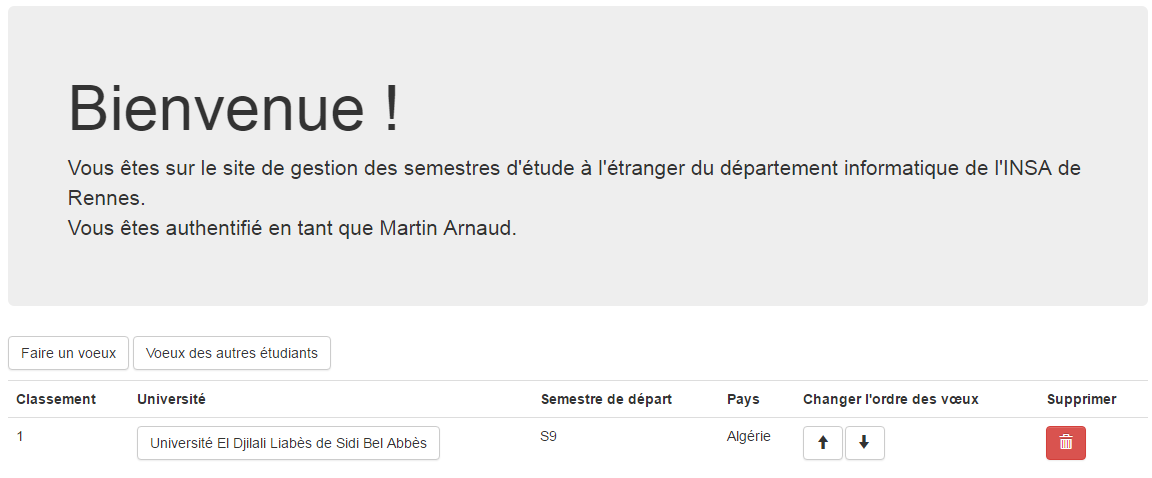
\includegraphics[width=16cm,height=9cm]{Images/Etudiant/faire_voeux_etud.png}
  	\caption{Accueil étudiant: phase de vœux}
  \end{figure}
            
    \begin{enumerate}
       	\item accès à la liste des universités dans laquelle les élèves sélectionnent leurs vœux (cf \ref{listuniv}),
       	\item lien vers la liste des étudiants de votre département avec leurs vœux ordonnés,
       	\item lien vers l'université,
       	\item flèches permettant de changer l'ordre d'un vœux (monter ou descendre l'ordre de priorité du vœux).
     \end{enumerate}
     
  \begin{figure}[H]
   	\centering
     		
  	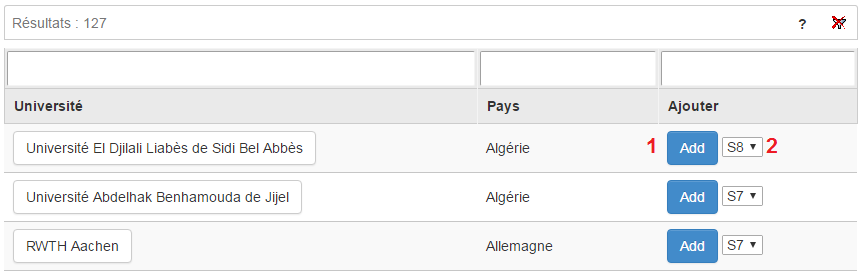
\includegraphics[width=16cm,height=5cm]{Images/Etudiant/liste_univ.PNG}
   	\caption{Liste des universités accessibles}
   	\label{listuniv}
  \end{figure}
  
 	\begin{enumerate}
	 \item ajoute l'université aux vœux (en dernière position),
	 \item choix du semestre de départ.
	\end{enumerate}


  \subsection{Accueil étudiant: phase dépôt de contrat d'étude}
	\label{pl}  
  \begin{figure}[H]
  	\centering
  	
  	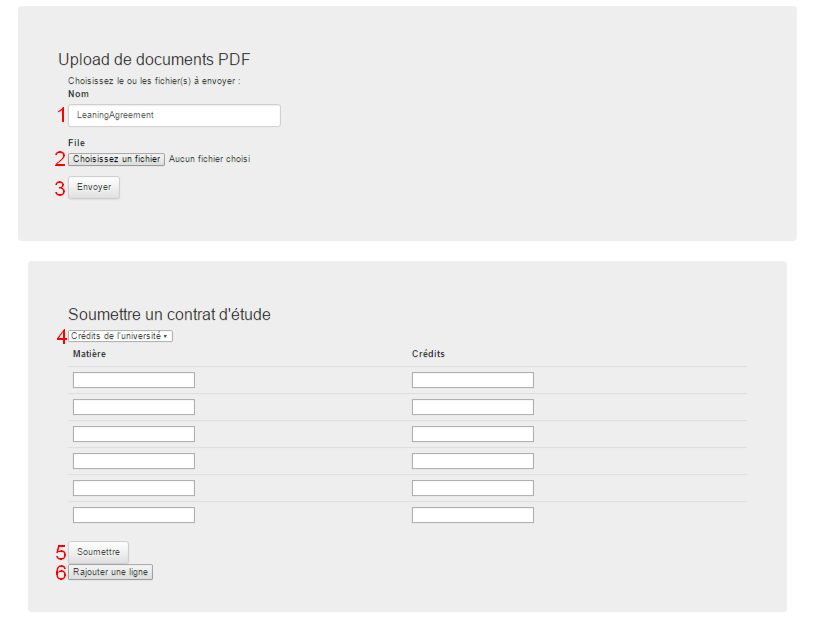
\includegraphics[width=16cm,height=9cm]{Images/Etudiant/learning_etud.png}
  	\caption{Accueil étudiant: phase dépôt de contrat d'étude}
  \end{figure}
  
    \begin{enumerate}
    	\item nom descriptif du fichier envoyé,
    	\item accès à l'explorateur de fichiers de l'utilisateur et sélection du fichier à déposer (format pdf),
    	\item envoi du fichier (cf \ref{depfich}),
    	\item choix du type de crédit de la destination et remplissage du contrat (cf \ref{propce}),
    	\item envoi du contrat d'étude à valider,
     	\item ajout d'une ligne au contrat d'étude si nécessaire.
    \end{enumerate}

  \subsection{Accueil étudiant: phase de dépôt de notes}
   	\label{pn}
  \begin{figure}[H]
  	\centering
  	
  	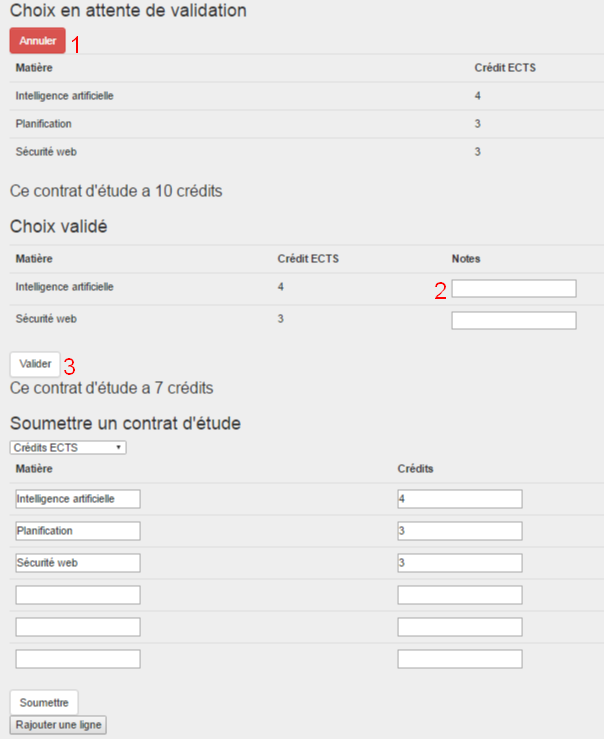
\includegraphics[width=14cm,height=12cm]{Images/Etudiant/notes_etud.png}
  	\caption{Accueil étudiant: phase de dépôt de notes}
  \end{figure}

    \begin{enumerate}
    	\item suppression d'un contrat d'étude proposé qui n'a pas encore été validé,
    	\item ajout des notes au contrat d'étude qui a été validé (cf \ref{depnot}),
    	\item envoi des notes rentrées.
    \end{enumerate}


\section{Choix des destinations}

Depuis la page d'accueil, cliquez sur "Faire un vœux". Une fois sur la page "Liste des Universités", en face de l'université souhaitée, sélectionnez le type de mobilité que vous voulez dans le menu déroulant puis cliquez sur "Add" pour l'ajouter à votre liste de vœux.   
 
\section{Gestion des vœux}

Depuis la page d'accueil, grâce aux bouton à droite de vos vœux, vous pouvez modifier l'ordre de vos vœux ou en supprimer.

\section{Proposition de contrat d'étude}
\label{propce}
Depuis la page d'accueil, dans la section "Soumettre un contrat d'étude", sélectionnez le type de crédit ayant cours dans votre université d'accueil puis entrez le nom des matières et le nombre de crédits rapportés par la matière.
Il est ensuite possible, en répétant la même manipulation, de soumettre d'autres contrats d'études.

\section{Dépôt de fichiers}
\label{depfich}
Depuis la page d'accueil, dans la section "Upload de documents", vous pouvez ajouter des fichiers pour l'élève en question. Pour cela, entrez le nom souhaité pour le document puis cliquer sur "choisissez un fichier" et sélectionnez le fichier. Cliquez enfin sur "envoyer" 

\section{Dépôt de notes}
\label{depnot}
Depuis la page d'accueil, dans la section "Choix validé", remplissez la case note correspondant à chaque matière avec soit des nombres (non-entiers), soit des lettres. Cliquez ensuite sur valider pour envoyer ces notes. Elles seront vérifiée par vos responsables RI en comparant à votre relevé de note, que vous déposerez sur le site.